\documentclass[11pt, a5paper]{book}

% This is a transcription done by Mairi Dulaney of Seattle, WA

% chktex-file 18

\usepackage{amsmath}
\usepackage{caption}
\usepackage[english]{babel}
\usepackage[T1]{fontenc}
\usepackage[]{geometry}
\usepackage{textcomp}
\usepackage{gensymb}
\usepackage{graphicx}
\graphicspath{{images/}}
\usepackage[utf8]{inputenc}
\usepackage{pgfplots}
\usepackage{titlesec}

\usepackage[activate={true,nocompatibility},final,tracking=true,kerning=true,factor=1100,stretch=10,shrink=10]{microtype}

\usepgfplotslibrary{fillbetween}
\usetikzlibrary{patterns}
\pgfplotsset{compat=1.16,samples=100}

\geometry{a5paper}
\nonfrenchspacing
\titleformat{\chapter}[display]
{\bfseries\Large}
{\centering
  \textsc{Chapter} \thechapter.} % label
{0.5ex}
{
  \vspace{1ex}
  \centering
  \scshape
}
[\vspace{-1ex}]

\titleformat{\section}[runin]{\bf}{\enspace}{0em}{}

\overfullrule=2cm


\begin{document}
\renewcommand{\thechapter}{\Roman{chapter}}
\title{Naval Reciprocating Engines and Auxiliary Machinery}
\author{Barton and Stickney}
\date{1914}
\maketitle


\chapter{Work---Energy---Power}
\section{Work} consists in overcoming resistance through space; the
result of the exertion of force through a certain distance.  In order
that work may be done there must be, not only a force, but also a
motion.\par

\section{Energy} is defined as the power or capacity of bodies for
doing work, and a body has more energy the more work it can do without
regarding time.  A force acting through space can be said to exert
energy, but when this is applied and a resistance overcome through a
certain distance, then work is done.\par

The unit of work is the \textit{foot-pound}, or the work done by a
force of one pound acting through the space of one foot; thus 10
pounds raised through a distance of 5 feet, or a pressure of 5 pounds
exerted through 10 feet, produces in either case 50 foot-pounds of
work.  The \textit{foot-ton} or \textit{inch-ton} is sometimes
employed for convenience in special cases and is the work of lifting
one ton through one foot or one inch.  The unit of work has no
reference to the time taken, for the same amount of work is done in
overcoming the resistance whether it can be done in one minute or one
hour.\par

From the definition of the unit of work it follows that the work done
by a body equals the product of the mean force of resistance in
pounds, and the distance moved in feet.  Hence, it may be represented
by the \textit{area} of a closed \textit{figure}, which is also the
product of two quantities, the mean altitude representing the mean
resistance force, and the length, the space or distance moved through.
This is known as a \textit{work diagram} and is the method practically
applied in measuring the work done by engines, and for which the
indicator is used.  (See Chapter X, The Indicator and the Indicator
Diagram.)\par

\section{Power.}The power of an engine involves the element of time,
and is measured by the rate at which it can do work, and is the amount
of work done in a unit of time.\par

In engineering calculations, the unit of power adopted is the
\textit{horse power} which represents the performance of 33,000
foot-pounds of work per minute or 550 foot-pounds of work per second.
Since the heat unit is equal to 778 units of work, one horse power is
equal to $33,000 \div 778 = 42.42$ B. T. U. per minute.\par

\begin{equation*}
  Horse\:Power = \frac{Work\:done}{33,000 \times time\:in\:minutes.}
\end{equation*}

\section{Energy} is defined as the capacity for doing work and must not
be confused with \textit{Power}.  A body is said to contain more
energy the more work it can do regardless of time.  One ton of coal on
being burnt in the furnace of a boiler can produce steam for
developing, say 700 horse power in one hour, whereas in another
smaller boiler it can produce 50 horse power for 14 hours.\par

Energy, whether heat energy or any other, cannot be destroyed.  It can
take different forms, but according to the principle of the
\textit{Conservation of Energy}, the total of the energy remains the
same; the heat carried to the engine in the steam is transformed into
work, some passes to waste in various ways, but the sum of the heat
usually employed plus the heat carried to waste always equals
precisely the heat evolved from the source.\par

\section{Efficiency.}Of the entire energy received by an engine,
some is utilized in the production of useful work and the rest is lost
or wasted, in overcoming the friction for instance, and in various
other ways.  The ratio of useful work done to that of the energy
supplied is known as efficiency; thus in the case of a steam plant, it
is the ratio of the heat changed into work and the entire heat
supplied.\par

\begin{equation*}
  Efficiency = \frac{Useful\:work\:done}{Total\:energy\:received.}
\end{equation*}

In the motive power of a ship the final work done is the effect in
driving the ship.  Compared with the heat energy contained the fuel
consumed in this operation, the work done will be found to be but a
small fraction, and is due to the various losses from the boiler
through the mechanism to the propeller.  These losses are made up of
(1) losses in the boiler, (2) of the heat carried to waste in the
steam itself after leaving the boiler, (3) losses in the mechanism,
and (4) propeller losses.  The total efficiency of the propelling
apparatus is the product of the factors representing the efficiencies
of these four elements.  Any gain in the efficiency of on part results
in a corresponding gain in the general economy of the whole
machine.\par

In the text-book on Naval Boilers, it has been shown that the
principal losses in the boiler are due to incomplete combustion,
condensation, radiation, and high temperature of smoke-pipe gases, so
that only 60 to 70 per cent of the total energy of the fuel is
converted into useful work.  After steam leaves the boiler further
losses are experienced as the steam traverses the cylinders, due to
radiation, incomplete expansion, the action of the cylinder walls, and
principally the heat carried to waste in the condenser.  The ratio of
the effective work performed on the piston to the total heat contained
in the steam does not amount to more than from 10 to 20 per cent.\par

All the work made available by the steam driving the piston does not
reach the propeller, owing to losses in the mechanism, such as
frictions, etc., the energy wasted in this operation amounting to
about 20 per cent, leaving for the efficiency of the mechanism about
80 per cent.  Of the work now left to drive the propeller not more
than 50 or 60 per cent is utilized in overcoming the resistance to the
vessel and driving her ahead, owing to the losses in frictional and
edgewise resistance of the water on the blades, augment of resistance
and slip.\par

From the efficiencies given for the several stages from the boiler to
the propeller, it will be seen that the maximum efficiency of the
entire propelling machinery under the present conditions does not
exceed 5 or 6 per cent.\par

In the succeeding chapters will be taken up the causes of the losses
in the steam, mechanism, and propeller; to what extent they are
unavoidable; and the means taken to reduce them to a minimum.\par

Before proceeding to discuss the action of the steam in an engine, an
elementary description of its parts is essential in order to
understand the mechanism used in the conversion of the heat energy of
the steam into the work of driving the engine.\par

In Fig. 1, steam from the boiler is conveyed through the steam pipes
to the engine stop valve \textit{T}.  From \textit{T} a certain
quantity goes through the \textit{main valve v} into the
\textit{cylinder} 1, and there exerts energy against a \textit{piston
 P}.  By suitable mechanism, called the \textit{valve gear},
\textit{v} is actuated to admit steam to one end of the cylinder and
to allow it to escape or \textit{exhaust} from the other end, the
piston \textit{P} being moved by the steam during this time from one
end of the cylinder to the other.  This \textit{reciprocating motion}
of \textit{P} is converted outside of the cylinder by suitable
mechanism into a \textit{turning motion} of the shaft \textit{a}, to
the end of which is secured the \textit{propeller}.  The water in
which the latter turns and engine friction form the chief resistance
which the steam acting on \textit{P} has to overcome.\par

\begin{figure}[ht]
  \centering
  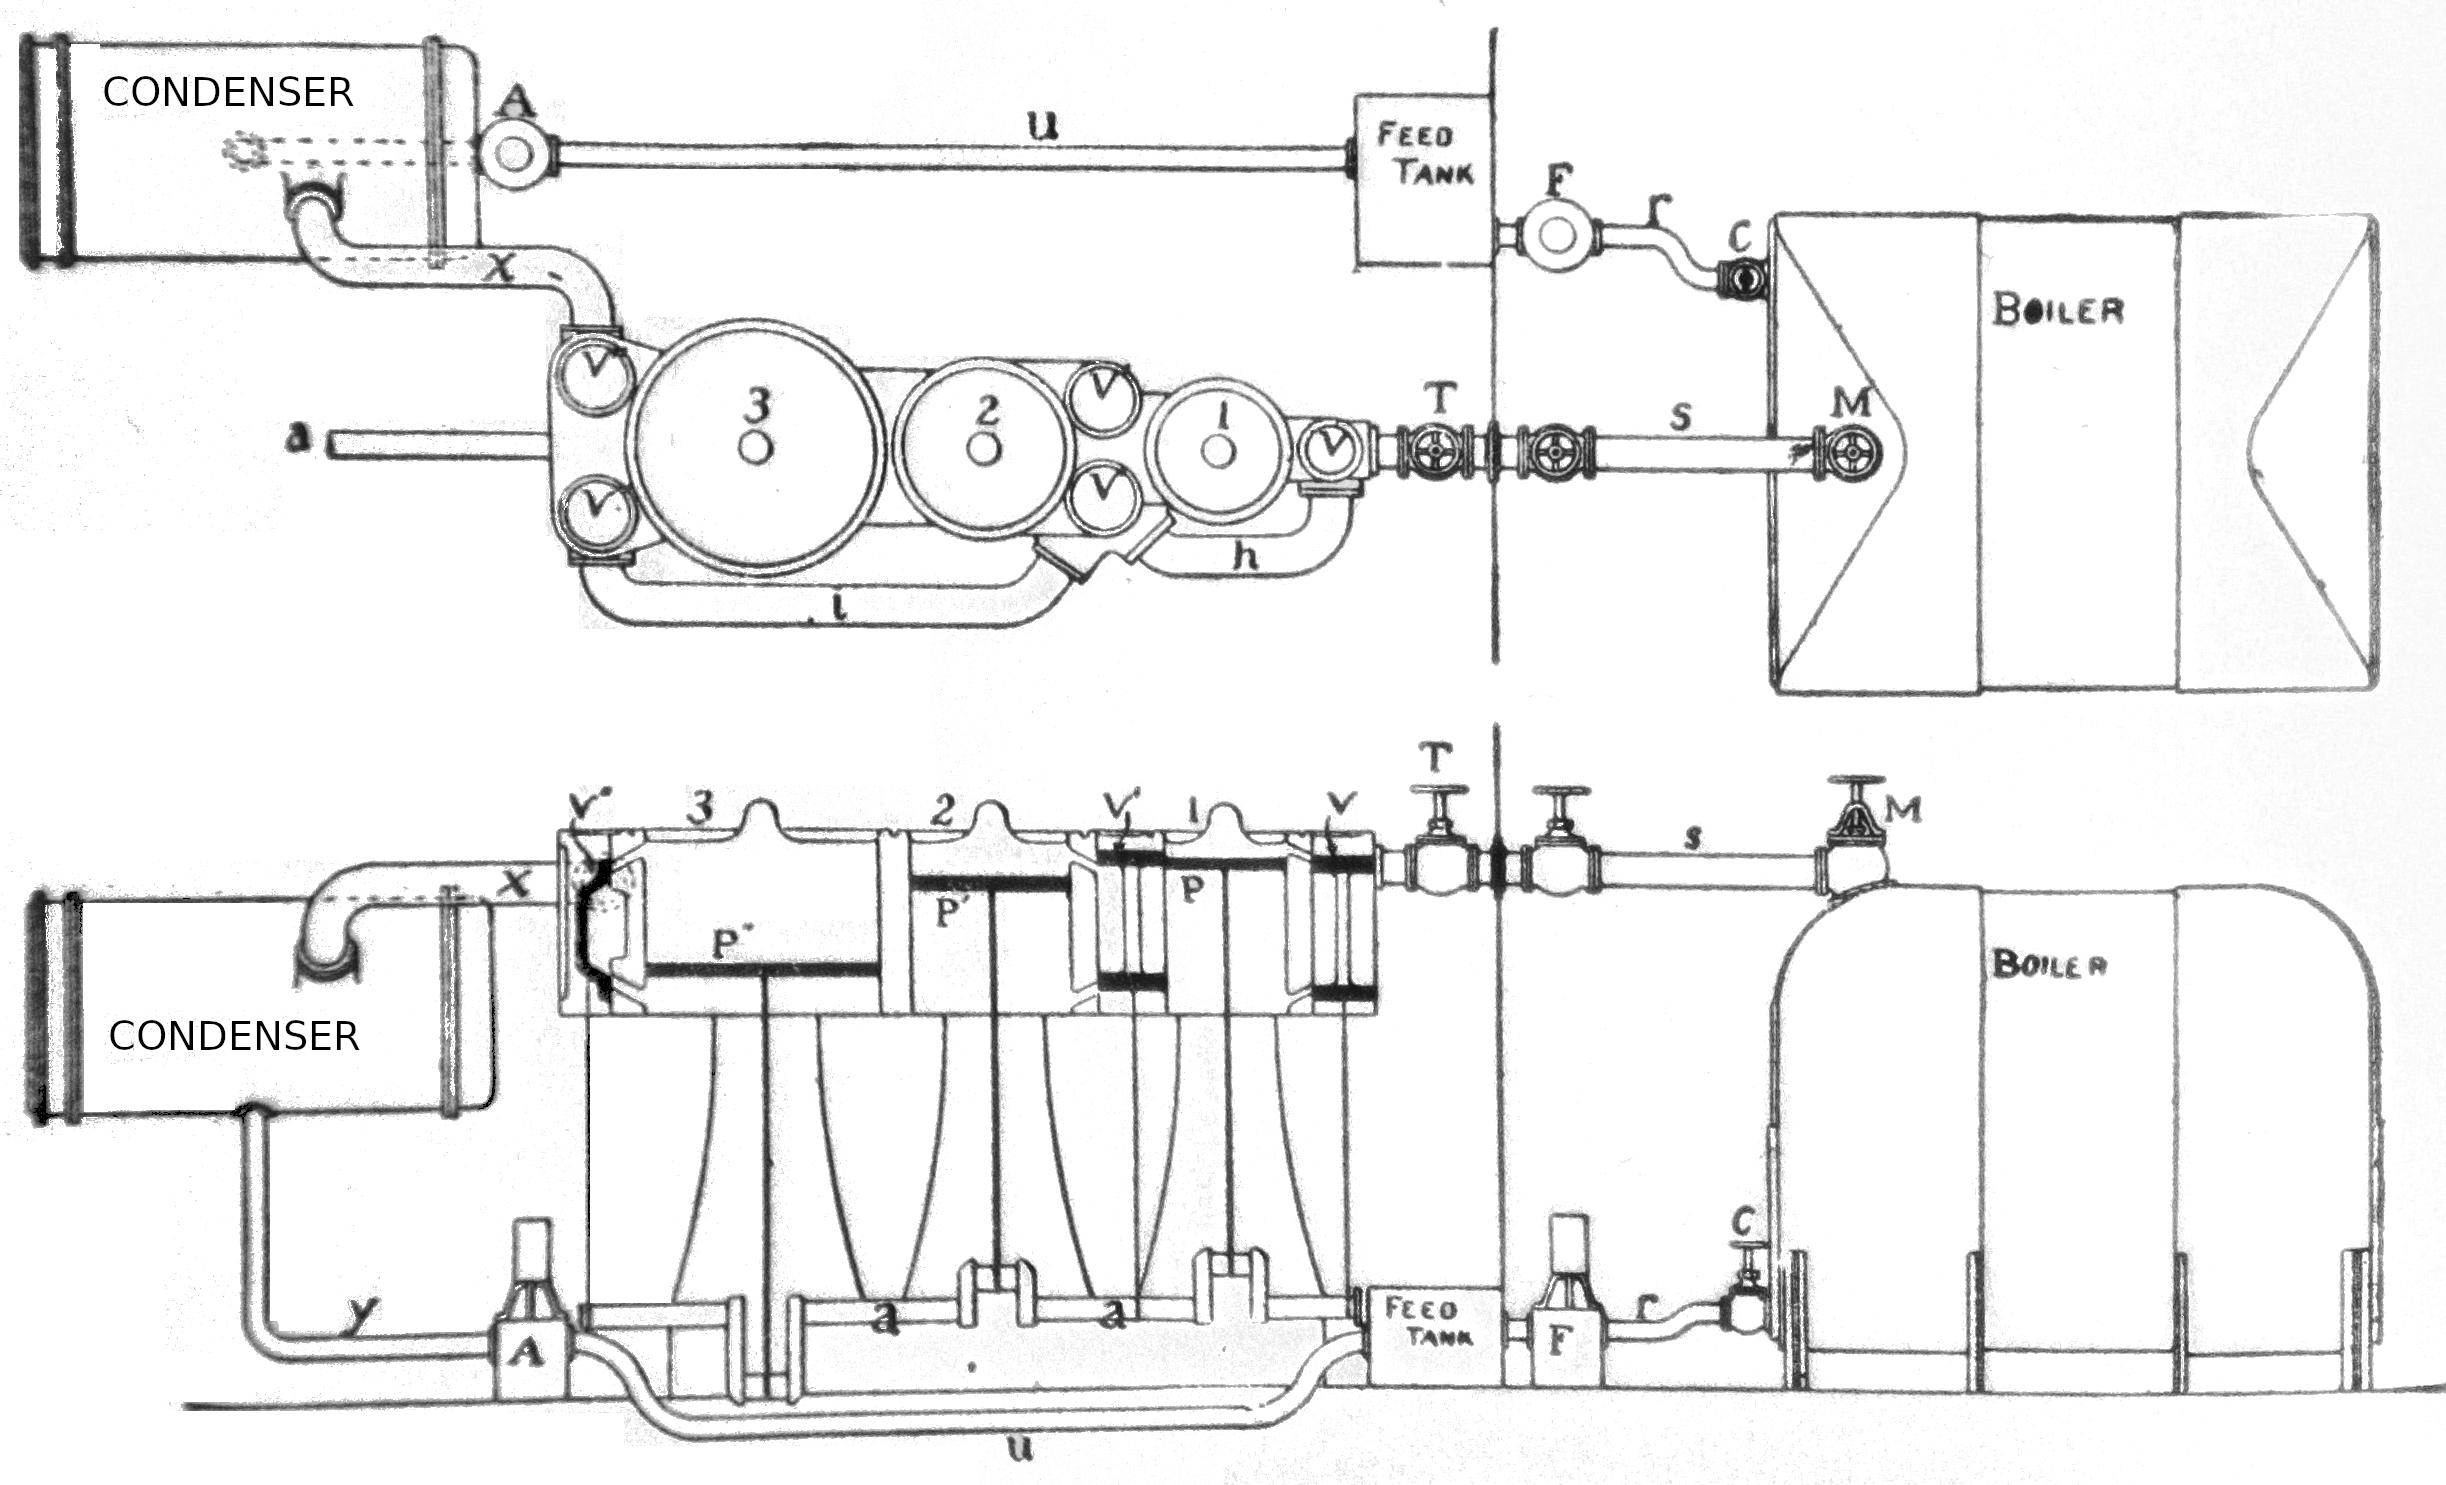
\includegraphics[scale=0.5]{fig_1.jpg}
  \caption*{\textsc{Fig.\ i.}}
\end{figure}

After acting on \textit{P} in one direction throughout its
\textit{stroke}, or distance that \textit{P} can travel in the
cylinder, the original quantity of steam is exhausted through one or
more additional cylinders into the \textit{condenser}, or it may be
exhausted from cylinder 1 direct into the condenser, or, more
directly, into the atmosphere.  In this last case, the engine is
called \textit{non-condensing}.\par

If only one cylinder and a condenser are used, they form a
\textit{simple condensing engine}.  When more than one is used, each
has its valve, piston, and other mechanism, the steam going through
the same action in each cylinder successively.  The cylinders, valves,
and pistons increase in size for each additional cylinder, and a
condenser is always used, the reasons for which will be shown later.
The pipes, \textit{h}, \textit{i} and other spaces connected the
exhaust side of one cylinder to the steam admission of the next,
\textit{are called receivers}.\par

Engines in which the steam passes successively through two, three, or
four cylinders are called \textit{double}, \textit{triple}, and
\textit{quadruple} expansion engines, the first one being commonly
called a \textit{compound} engine.  The cylinder which receives the
boiler steam is called the \textit{high-pressure} cylinder, and that
which exhausts it into the condenser, the \textit{low-pressure}
cylinder.  The cylinders between these two are called
\textit{intermediate-pressure} cylinders.  The various cylinders are
designated by the explanatory letters, H. P., I. P., and L.P\@.  For a
quadruple expansion engine, the I. P. cylinder next to the H. P. is
designated the 1st I. P., and the next one as the 2d I.P.\par

In the condenser, the steam is converted into water, which with any
air is removed by means of the \textit{air pump A} and returned to the
boiler through a \textit{feed tank} and by the \textit{feed pump F}.\par

\chapter{The Action of the Steam.}

From the definition, the efficiency of the steam is simply the ratio
of the energy exerted by the steam to the heat required to produce it,
and since the difference between the amounts of heat utilized to
obtain the same weight of steam at different pressures is so slight,
the question of economy is only that of obtaining the greatest amount
of work from a given weight of steam.\par

From the formula for total heat of steam, it will be seen that the
amount of heat required to convert one pound of water from a
temperature of 100\degree{} into steam of 60 pounds pressure, is about
1115 thermal units, and to convert the same quantity of water, at the
same temperature, into steam at 200 pounds pressure, is 1140 thermal
units, only $2\frac{1}{2}$ per cent greater heat required for three
times the pressure.  This fact is utilized in modern engines by the
employment of high pressures and expansion, with a consequent increase
of work from the same weight of steam.\par

A well-known formula and theorem of thermodynamics, showing the
maximum efficiency of steam, is represented by\par

\begin{equation*}
  E = \frac{T_1 - T_2}{T_1} = \frac{t_1 - t_2}{t_1 + 461}
\end{equation*}

\noindent{} where $T_1 =$ initial absolute temperature; $t_1 =$
initial temp. F.; $T_2 =$ final absolute temperature; $t_2 =$ final
temperature F.\par

That is, the greatest possible efficiency of any heat engine depends
only upon the highest and lowest temperatures between which it is
worked, and is independent of the nature of the working substance.
The higher the temperature and pressure of the working fluid supplied
and the lower that at which it is rejected, the higher will be the
efficiency of the engine.\par

Taking the case of a modern engine working with saturated steam of an
initial pressure of 250 pounds per gauge, at the engine, approximately
265 pounds absolute, and exhausting into a condenser in which there is
an absolute pressure of 3 pounds per square inch, approximately equal
to a vacuum of 24 inches, the corresponding initial and final
temperatures will be 401\degree{}F. and 141\degree{}F., assuming that
there is no difference between the back pressure or pressure on the
exhaust side of the piston and the pressure in the condenser.\par

Then, Maximum Efficiency $=\frac{401 - 141}{862} = .301$.\par

That is, even if the total heat of the saturated steam admitted at a
temperature of 401\degree{}F. could be so utilized in work in the
engine, that, when the steam leaves the engine, it would carry away
only the total heat due to the temperature of 141\degree{}F., the
greatest possible amount of heat utilized would be only about
one-third of that supplied.  It would be, therefore, impossible to
reduce the loss, even in an ideally perfect engine, below 70 per cent
for the temperature range given above.  But in the actual engine the
ideal conditions are not reached, due to losses which will be taken up
later, so that instead of a loss of 70 per cent, practically it
amounts to 75 or 85 per cent, making the efficiency of a good steam
engine only from 15 to 25 per cent.\par

\section{Methods of Increasing Efficiency.}To increase the range of
temperature and hence the efficiency, the value of $t_1$ has been
successively raised, as boilers could be designed to withstand the
increased pressures, from the former low pressures of 25 and 30 pounds
up to 250 and 300 pounds of the present day.  In looking for a
reduction of $t_2$, it is impossible with a non-condensing engine, or
one exhausting into the atmosphere, to obtain a much smaller back
pressure than 18 or 19 pounds absolute, or 3 to 4 pounds above the
pressure of the atmosphere, owing to the friction in pipes and
passages and the speed of the engine.  The lower value of $t_2$ in the
non-condensing engine is consequently limited to 220\degree{} F.\par

In the condensing engine, however, in which the exhaust steam is
discharged into a condenser, and condensed by cooling water, the
temperature and pressure are both lowered.  The back pressure in this
case falls to about 3 pounds absolute and a corresponding temperature
of about 141\degree{} F.  The difference between the back pressure and
that of the atmosphere is called a vacuum and is measured in inches of
mercury.\par

As an example of this saving by the use of a condenser, let the
initial steam have a pressure of 250 pounds absolute with a
corresponding temperature of 401\degree{} F.\par

For non-condensing $E = \frac{401-220}{401+461}=.209$.\par\label{cond_non-cond}

For condensing $E=\frac{401-141}{401+461}=.301$.\par

Or the efficiency of the steam has been increased 45 per cent by the
installation of a condenser.\par

The above result can be shown graphically by means of the indicator
diagram.  This diagram is obtained from an instrument attached to the
cylinders of an engine and shows the pressures in the cylinders at
varying points of the stroke, and many other facts of importance
regarding the action of the steam within the cylinder. (See chapter
X.)\par

The theoretical form of an indicator diagram taken from a condensing
engine, in which a gas such as superheated steam is used, the back
pressure assumed constant throughout the stroke and the admission and
exhaust of steam instantaneous, is shown in Fig. 2.\par

Ordinates represent the steam pressures while the abscissa represents
the volume.  Since the volume of a cylinder is the product of the
stroke and and area of piston, the line of volume may also be used for
the stroke.\par

Let \textit{OV} represent the \textit{stroke} of the engine.  The
vertical \textit{admission line} on the left shows the rise of
pressure and \textit{OP} represents the absolute initial pressure on
the piston.  As the piston moves with this pressure constantly upon
it, the horizontal \textit{steam line PA} is traced; at \textit{A} the
admission of steam is cut off by the valve closing the steam port.
Expansion commences at \textit{A}, the piston being driven forward by
the expansive action of the steam, and the pressure falling as the
volume increases.  This period is represented by the \textit{expansion
  line AB}.  Had the steam followed with full steam pressure to the
end of the stroke, the admission line would have been carried to
\textit{A'}.  At \textit{A'} (for a non-expansive) or \textit{B} (for
an expansive engine) the exhaust valve opens to the atmosphere or
condenser as the case may be and the pressure falls to the final one
as shown \textit{VK} or \textit{VE}.  The piston now begins to return,
steam of initial pressure being admitted to the other side, and the
steam escapes against the back pressure \textit{VK} or \textit{VE}
until the end of the return stroke at \textit{O}.  For a condensing
engine, \textit{DE} is called the back pressure line.  The exhaust now
closes and live steam is again admitted and the operation repeated for
each stroke.\par

By closing the indicator cock to the cylinder and opening to the
atmosphere, the atmospheric line \textit{GH} is drawn.\par

\begin{figure}[h]
  \centering
  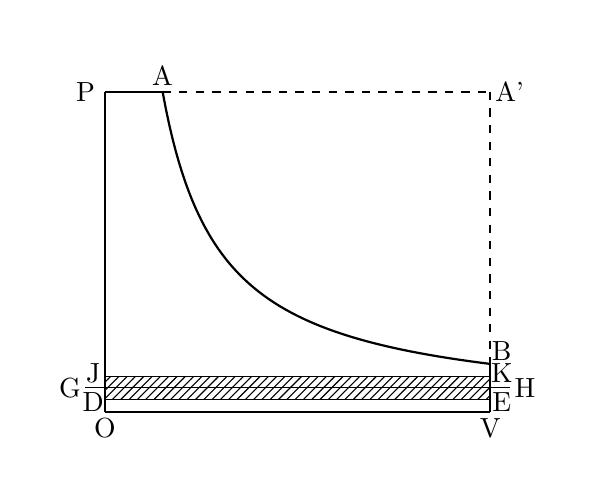
\begin{tikzpicture}
    \begin{axis}[
        ticks=none,
        xmin=-2,
        xmax=12,
        ymin=-2,
        ymax=12,
        axis x line=none,
        axis y line=none,
      ]
      \addplot[black,thick, domain=1.5:10]{15/x};
      \addplot[black, thick, domain=0:10]coordinates{(0,10)(1.5,10)};
      \addplot[black, thick, domain=0:10]coordinates{(10,0)(10,1.5)};
      \addplot[black, thick, domain=0:10]coordinates{(10,0)(0,0)};
      \addplot[black, thick, domain=0:10]coordinates{(0,0)(0,10)};
      \addplot[black, thick, dashed, domain=0:10]coordinates{(1.5,10)(10,10)};
      \addplot[black, thick, dashed, domain=0:10]coordinates{(10,10)(10,1.5)};
      \addplot[black, name path=ncbp, thin, domain=0:10]coordinates{(0,1.1)(10,1.1)};
      \addplot[black, name path=cbp, thin, domain=0:10]coordinates{(0,.4)(10,.4)};
      \addplot[black, thin, domain=-1:11]coordinates{(-.5,.75)(10.5,.75)};
      \addplot[thick, color=black, fill=black, pattern=north east lines,]
        fill between[of=ncbp and cbp, soft clip={domain=0:10},];
      \node at (axis cs:10.5,10) {A'};
      \node at (axis cs:1.5,10.5) {A};
      \node at (axis cs:-.5,10) {P};
      \node at (axis cs:-.3,1.2) {J};
      \node at (axis cs:-.9,.75) {G};
      \node at (axis cs:-.3,.3) {D};
      \node at (axis cs:0,-.5) {O};
      \node at (axis cs:10,-.5) {V};
      \node at (axis cs:10.3,.3) {E};
      \node at (axis cs:10.9,.75) {H};
      \node at (axis cs:10.3,1.2) {K};
      \node at (axis cs:10.3,1.9) {B};
    \end{axis}
  \end{tikzpicture}
  \caption*{\textsc{Fig.\ 2.}}
\end{figure}

In engine calculations, the pressures used are absolute steam
pressures or pressures measured from the zero line or line of no
pressure, and should be distinguished from \textit{pressures by
  gauge}, which latter are simply steam pressures above that of the
atmosphere, and are those pressures indicated by the readings on the
ordinary pressure gauges.\par

Since the indicator diagram is merely a diagram of work, its length
shows the distance moved through by the piston, while the effective
force is the excess of the mean forward pressure against the piston on
one side, during admission and expansion, above the mean back pressure
on the other side, as the exhaust steam passes to the condenser.
Hence the area of the entire diagram \textit{OPABV}, minus the area of
back pressure \textit{ODEV}, represents to scale the effective work
done on one side of the piston.  A similar diagram taken from the
other end of the cylinder shows the work done on the other side during
the double stroke.\par

The area of this diagram, and consequently the work done with a given
\textit{weight of steam}, may be increased by decreasing the amount of
back pressure, \textit{i.e.}, lowering the back pressure line, also
by raising the steam and expansion lines.  The former can be done by
the use of a condenser and the latter by increasing the initial
pressure and using an earlier cut-off.\par

The comparative work of the two engines mentioned on
page~\pageref{cond_non-cond} can be shown by the diagram, Fig. 2,
since the initial pressure and the cut-off are the same, the only
difference in the cards from each each engine would be the position of
the back pressure line.  In the non-condensing engine this line would
be at \textit{JK}, and for the condensing engine at \textit{DE},
giving an increase in the area of the condensing engine diagram, and,
consequently, an increase in the work done represented by the area
\textit{JKED}.\par

\section{Definitions.}---\textit{Absolute Temperature}---Temperatures,
estimated not from the ordinary zero, but from a point 461\degree{}
below the zero of Fahrenheit's scale, are known as \textit{absolute
  temperatures}, and the point, ---461\degree{} F.\ is called the
\textit{absolute zero of temperature}.\par

\textit{Absolute Pressure} is measured from the zero pressure of the
atmosphere or 14.7 pounds per square inch below the pressure of the
atmosphere when the mercury barometer stands at 30 inches.\par

\textit{Specific Volume}.---The specific volume of steam is the number
of cubic feet contained in one pound of steam at any given
pressure.\par

\textit{Relative Volume}.---The relative volume is the ratio which the
volume of steam produced bears to the volume from which it was
generated.\par

\textit{Ratio of Expansion} is the ratio which the volume of a given
quantity of steam bears to the volume it occupied before
expansion.\par

\textit{Saturated Steam} is steam at the greatest possible density for
its pressure.  Steam in this condition is just at the point of
condensation and any increase of pressure or decrease of temperature
will cause some of it to be condensed.  The temperature of saturated
steam is the temperature of the water with which it is in contact.
For each pressure of saturated steam there is a fixed temperature.
See "Saturated Steam Table" in Appendix.\par

Many formulae have been produced to represent the results of Regnault
and other experimenters on the relation between the pressure and the
temperature of saturated steam.  They are all of a complicated nature;
the simplest is probably the following:
$\log\; p=5\times\frac{t-212}{t+367}+\log\; 14.7$,
where \textit{p} is the
absolute pressure in pounds per square inch and \textit{t} is the
temperature in degrees Fahrenheit.\par

For ready numerical calculations, a steam table, such as given in the
Appendix, will be found more useful and convenient, but in the absence
of such a table the above formula can be used for all practical
purposes.\par

The relation between the pressure and the volume of saturated steam
may be approximately expressed by means of the formula:
$pv^\frac{17}{16} = 475$, or more accurately, $pv^1.0616 = 479$, where
\textit{p} is the absolute pressure in pounds per square inch and
/textit{v} is the volume in cubic feet.\par

\textit{superheated Steam}.---Steam \textit{free from the water} from
which it was generated and supplied with additional heat becomes
\textit{superheated} and approaches the condition of a perfect gas,
while the temperature and density no longer correspond with the
pressure as during evaporation.  The temperature of saturated steam in
the presence of water cannot be raised without raising its pressure,
but steam may be superheated without an increase of pressure, if it is
free from water and is allowed to expand as the heat is added.\par

\textit{Wet Steam}.---Ordinary steam carrying with it a greater or
less proportion of water, either in suspension or otherwise mixed with
it, is known as \textit{wet or moist steam}.  Wet steam will become
drier or saturated steam become superheated if it falls in pressure
without a corresponding loss of heat, as for instance, in the free
expansion of the exhaust steam to the receivers of a multiple
expansion engine.\par

\textit{Expansive Action of Steam}.---From the expansive property
which steam and other gases possess, a still further economy may be
obtained by the performance of increased work from the same weight
of steam.  By taking advantage of this property and cutting off the
supply of steam at some point before the completion of the stroke, the
steam will expand and continue to drive the piston with a gradually
decreasing pressure, until it is exhausted into the atmosphere or the
condenser.\par

If a volume of gas be admitted to a cylinder, it will fill the
cylinder and exert a definite pressure per square inch upon the
piston.  If the piston is moved so as to increase the volume, the
pressure on the piston will be less.  If the piston had been moved to
decrease the volume, the gas would have been compressed, its
\textit{density} or weight \textit{per cubic foot} have become
greater, and with a greater pressure per square inch upon the piston.
This action in the expansion of a perfect gas is expressed by Boyle's
law as follows:\par

"The volume of a given mass varies inversely as the pressure, provided
by the temperature be kept constant;" or the product of the pressure
\textit{p} and volume \textit{v} is constant, or $pv=constant$.\par


\begin{figure}[h]
  \centering
  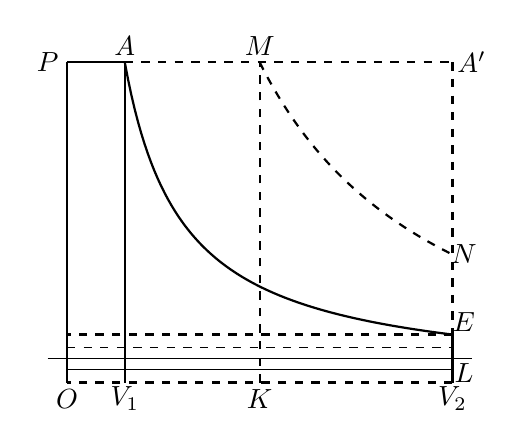
\begin{tikzpicture}
    \begin{axis}[
        ticks=none,
        xmin=-2,
        xmax=12,
        ymin=-2,
        ymax=12,
        axis x line=none,
        axis y line=none,
      ]
      \addplot[black, thick, domain=1.5:10]{15/x};
      \addplot[black, thick, domain=0:10]coordinates{(0,10)(1.5,10)};
      \addplot[black, thick, domain=0:10]coordinates{(10,0)(10,1.5)};
      \addplot[black, thick, dashed, domain=0:10]coordinates{(10,0)(0,0)};
      \addplot[black, thick, domain=0:10]coordinates{(0,0)(0,10)};
      \addplot[black, thick, dashed, domain=0:10]coordinates{(1.5,10)(10,10)};
      \addplot[black, thick, dashed, domain=0:10]coordinates{(10,10)(10,1.5)};
      \addplot[black, name path=ncbp, thin, dashed, domain=0:10]coordinates{(0,1.1)(10,1.1)};
      \addplot[black, name path=cbp, thin, domain=0:10]coordinates{(0,.4)(10,.4)};
      \addplot[black, thin, domain=-1:11]coordinates{(-.5,.75)(10.5,.75)};
      \addplot[black, thick, dashed, domain=0:10]coordinates{(10,1.5)(0,1.5)};
      \addplot[black, thick, domain=0:10]coordinates{(1.5,0)(1.5,10)};
      \addplot[black, thick, dashed, domain=0:10]coordinates{(5,0)(5,10)};
      \addplot[black, thick, dashed, domain=5:10]{60/x-2};
      \node at (axis cs:10.5,10) {$A'$};
      \node at (axis cs:1.5,10.5) {$A$};
      \node at (axis cs:-.5,10) {$P$};
      \node at (axis cs:0,-.5) {$O$};
      \node at (axis cs:10,-.5) {$V_2$};
      \node at (axis cs:10.3,.3) {$L$};
      \node at (axis cs:10.3,1.9) {$E$};
      \node at (axis cs:5, 10.5) {$M$};
      \node at (axis cs:5, -.5) {$K$};
      \node at (axis cs:1.5, -.5) {$V_1$};
      \node at (axis cs:10.3, 4) {$N$};
    \end{axis}
  \end{tikzpicture}
  \caption*{\textsc{Fig.\ 3.}}
\end{figure}



\end{document}
